
\chapter{Arquitetura de Software}
\label{sec-arquitetura}
\vspace{-1cm}

O sistema \emph{\imprimirtitulo} adota uma arquitetura de microserviços orientada a eventos e baseada nos princípios do modelo arquitetural proposto pelo \textbf{FrameWeb}, que organiza a aplicação em três camadas principais, \textbf{Presentation}, \textbf{Business} e \textbf{Data Access} e cinco pacotes, \textbf{View}, \textbf{Control}, \textbf{Application}, \textbf{Domain} e \textbf{Persistence}, como ilustrado na Figura~\ref{figura-arquitetura}. Essa abordagem permite estruturar a aplicação de forma modular, facilitando tanto a manutenção quanto a escalabilidade. 

A camada de \textbf{Presentation} corresponde à interface com o usuário, sendo composta pelos pacotes \textbf{View}, que concentram os arquivos relacionados ao \textbf{front-end}, como as páginas web desenvolvidas em componentes \textbf{Angular}, e \textbf{Control}, que reúnem as classes responsáveis por intermediar a comunicação com o framework \textbf{controlador frontal}. Nessa camada, a aplicação é um \textit{Single Page Application}, ou seja, uma implementação em que carrega apenas um único documento e, em seguida, atualiza o conteúdo do corpo desse documento \cite{mdn_spa}. Assim, o \textbf{front-end} é uma aplicação a parte do \textit{back-end}.

A camada de \textbf{Business} implementa as regras de negócio e os serviços da aplicação, enquanto a camada de \textbf{Data Access} é responsável pela persistência dos dados, utilizando o padrão \textbf{DAO}. A arquitetura é a de microsserviços orientada a eventos, que é viabilizada por meio do uso do \textbf{Kafka}, permitindo a comunicação assíncrona entre os microserviços. Segundo \citeonline{google_microservices}, "Uma arquitetura de microsserviços é um tipo de arquitetura em que o aplicativo é desenvolvido como uma coleção de serviços". Esses serviços serão desenvolvidos utilizando o \textit{framework} em Java \textbf{Spring Boot} e a linguagem \textbf{Go}, com os dados armazenados em bancos \textbf{MongoDB}, \textbf{PostgreSQL} e \textbf{DynamoDB} (na nuvem AWS)\footnote{https://aws.amazon.com}, além de \textbf{Redis} para mecanismos de cache e otimização de desempenho. Dessa forma, a arquitetura proposta segue os padrões definidos pelo \textbf{FrameWeb}, aliados a frameworks modernos e tecnologias robustas para suportar as demandas do sistema.

A Figura~\ref{figura-arquitetura} mostra a arquitetura do sistema em módulos baseados na arquitetura FrameWeb \emph{\imprimirtitulo} com microsserviços no Spring Boot (alguns serão em Go).

\begin{figure}[h]
	\centering
	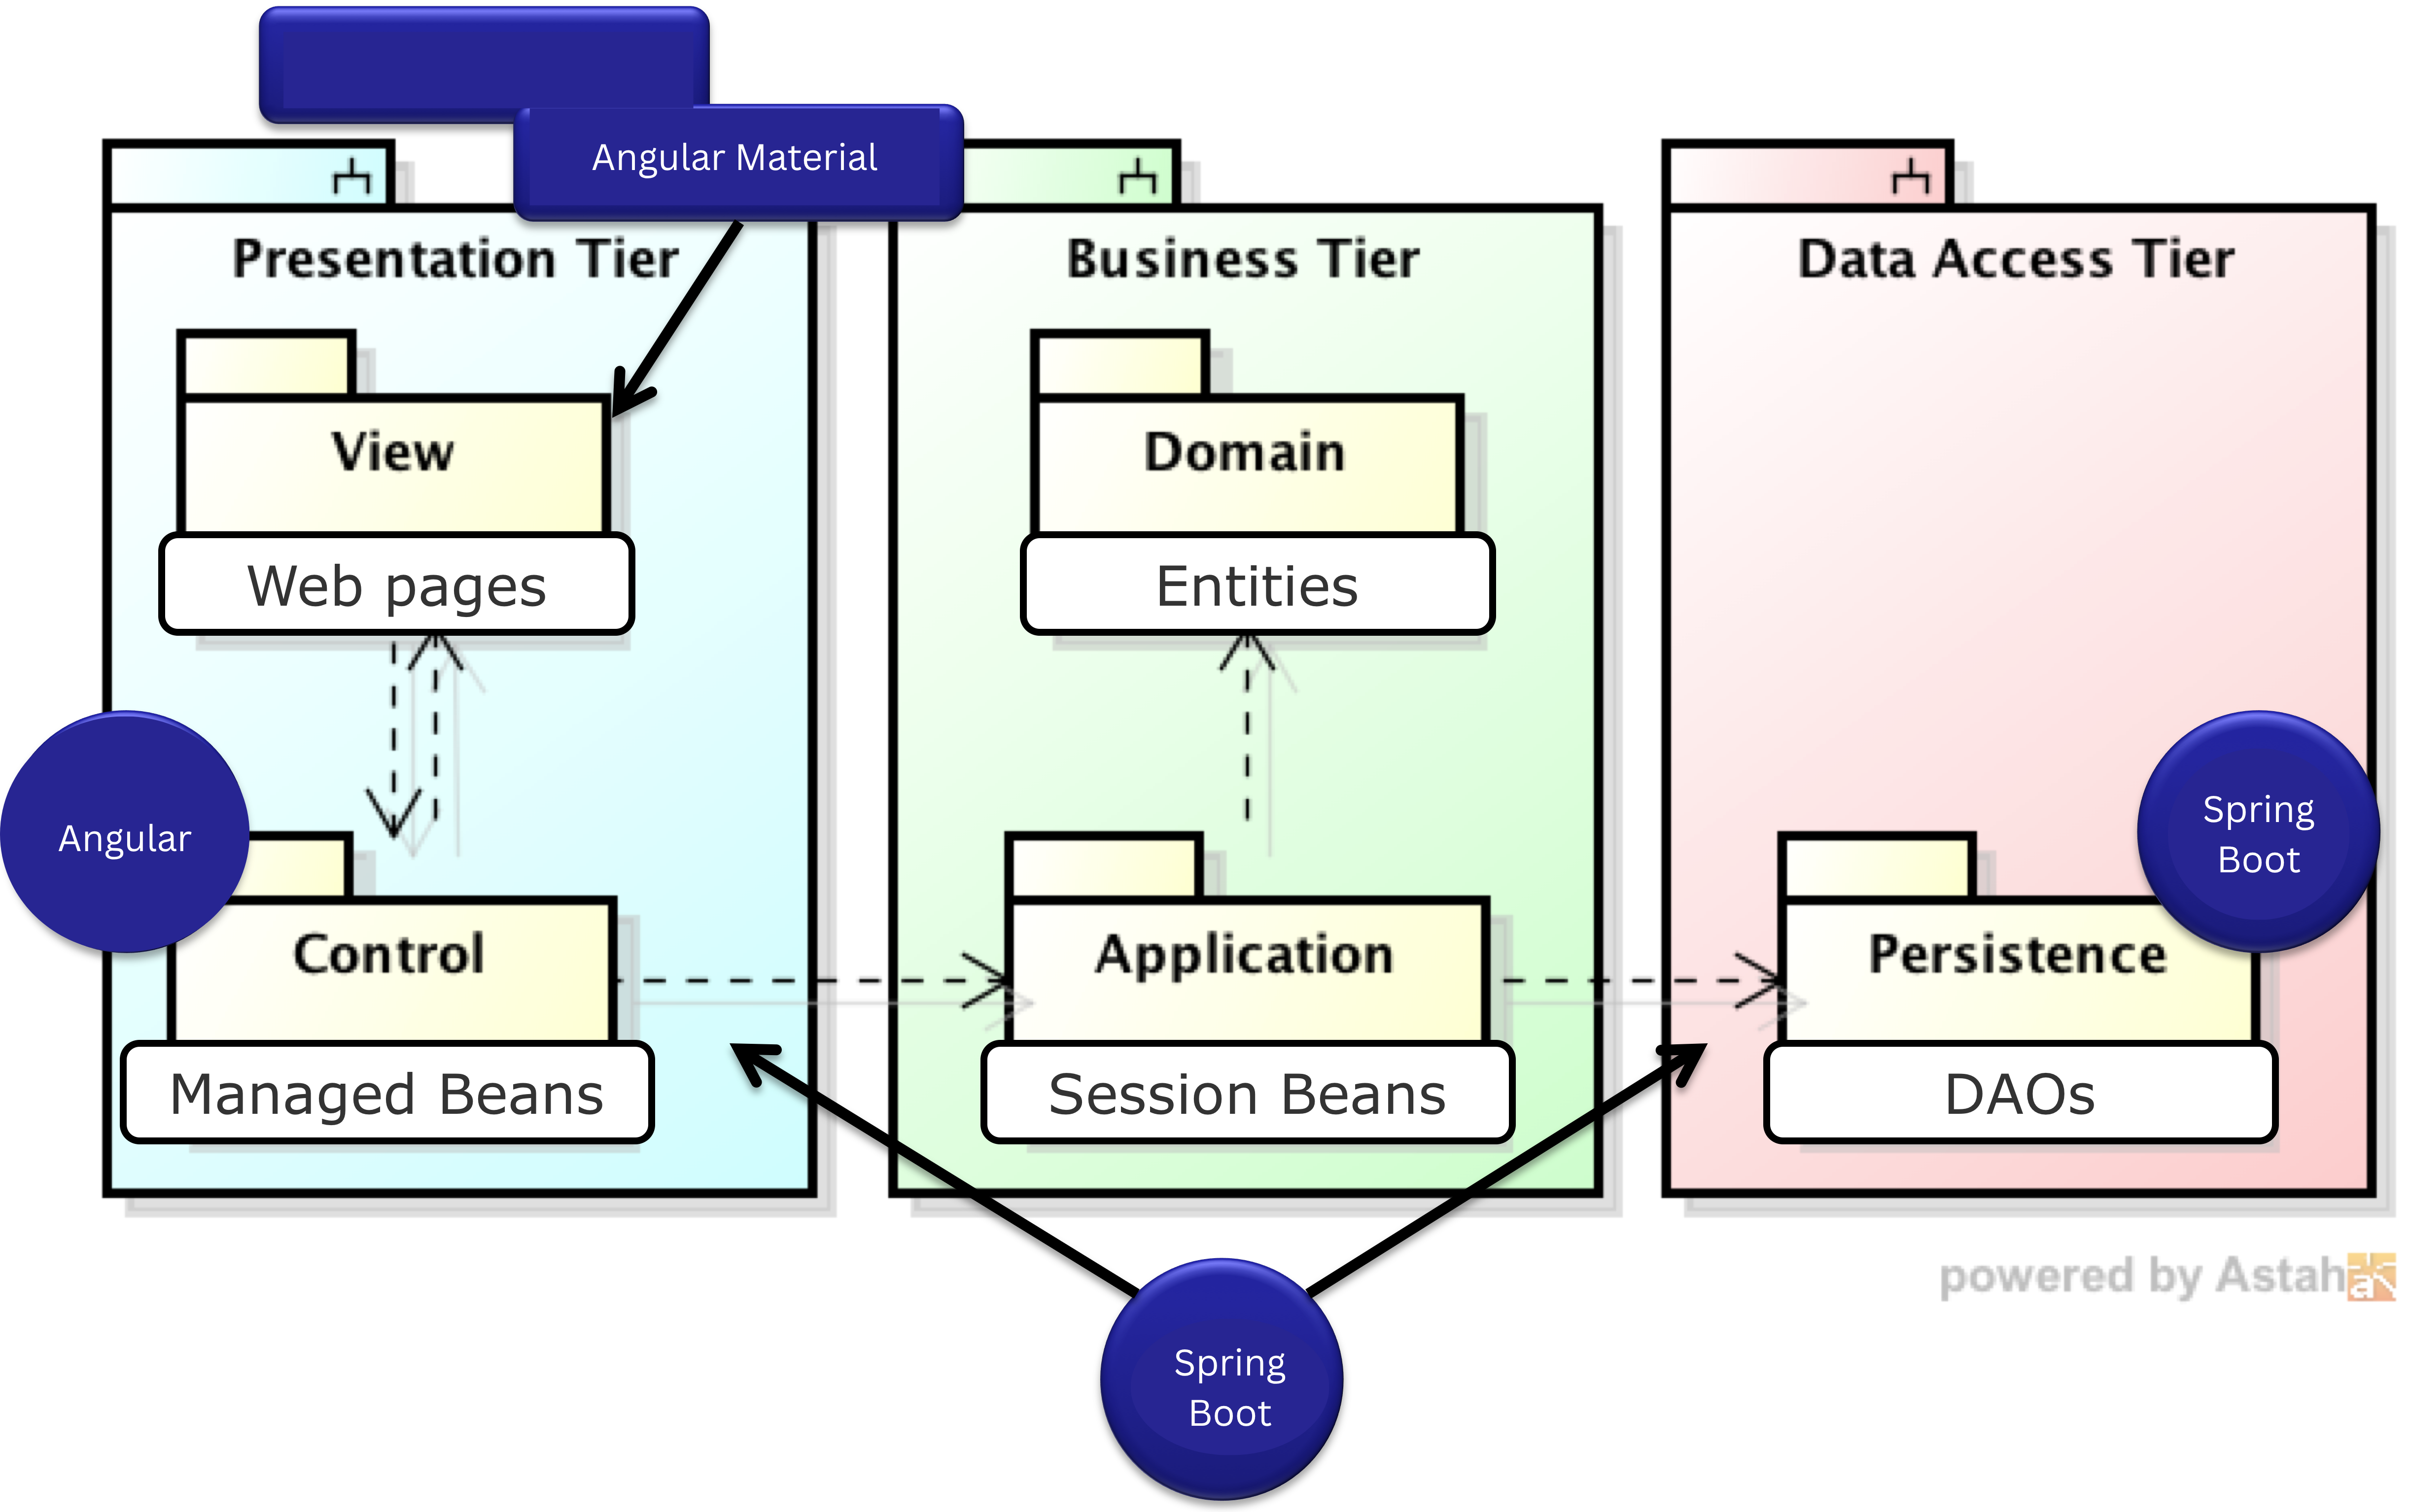
\includegraphics[width=0.8\textwidth]{figuras/arquitetura-frameweb.png}
	\caption{Arquitetura de Software.}
	\label{figura-arquitetura}
\end{figure}

A Figura~\ref{figura-arquitetura-campus} mostra a arquitetura de microsserviços orientada a eventos do back-end \emph{\imprimirtitulo}. Na figura o lado do front-end é abstraído por "Web" com a indicação do ícone do Angular. As requisições do front-end passam por um \textit{Gateway} utilizando o \textbf{Kong Gateway}, em que este direciona as requisições para os devidos microsserviços, fazendo o \textit{load balancing}, distribuindo a carga de requisições entre as instâncias de cada microsserviço. À direita do \textit{Gateway} estão os microsserviços representados por caixas múltiplas (indicando poder ter mais de uma instância) e com a tecnologia de implementação indicada pelo ícone do Spring Boot ou da linguagem Go. Cada microsserviço tem o seu banco de dados (também com indicação de ícones da tecnologia), para que os contextos e cargas não se misturem, com a exceção do \textit{Notification} em que sua responsabilidade é de enviar \textit{e-mails} através dos serviços \textbf{Amazon SES}. A comunicação entre o \textit{front-end} e \textit{back-end} se dá via \textbf{API RESTful}. O microsserviço \textit{Media} faz o envio das imagens cadastradas no sistema para o serviço em nuvem \textbf{Amazon S3} e armazena seus dados no banco \textbf{DynamoDB}, que também é um serviço da nuvem da \textit{Amazon}. Entre os microsserviços, a comunicação pode ocorrer de forma síncrona por \textit{API RESTful} ou de forma assíncrona pela \textit{Kafka}.

\begin{figure}[h]
	\centering
	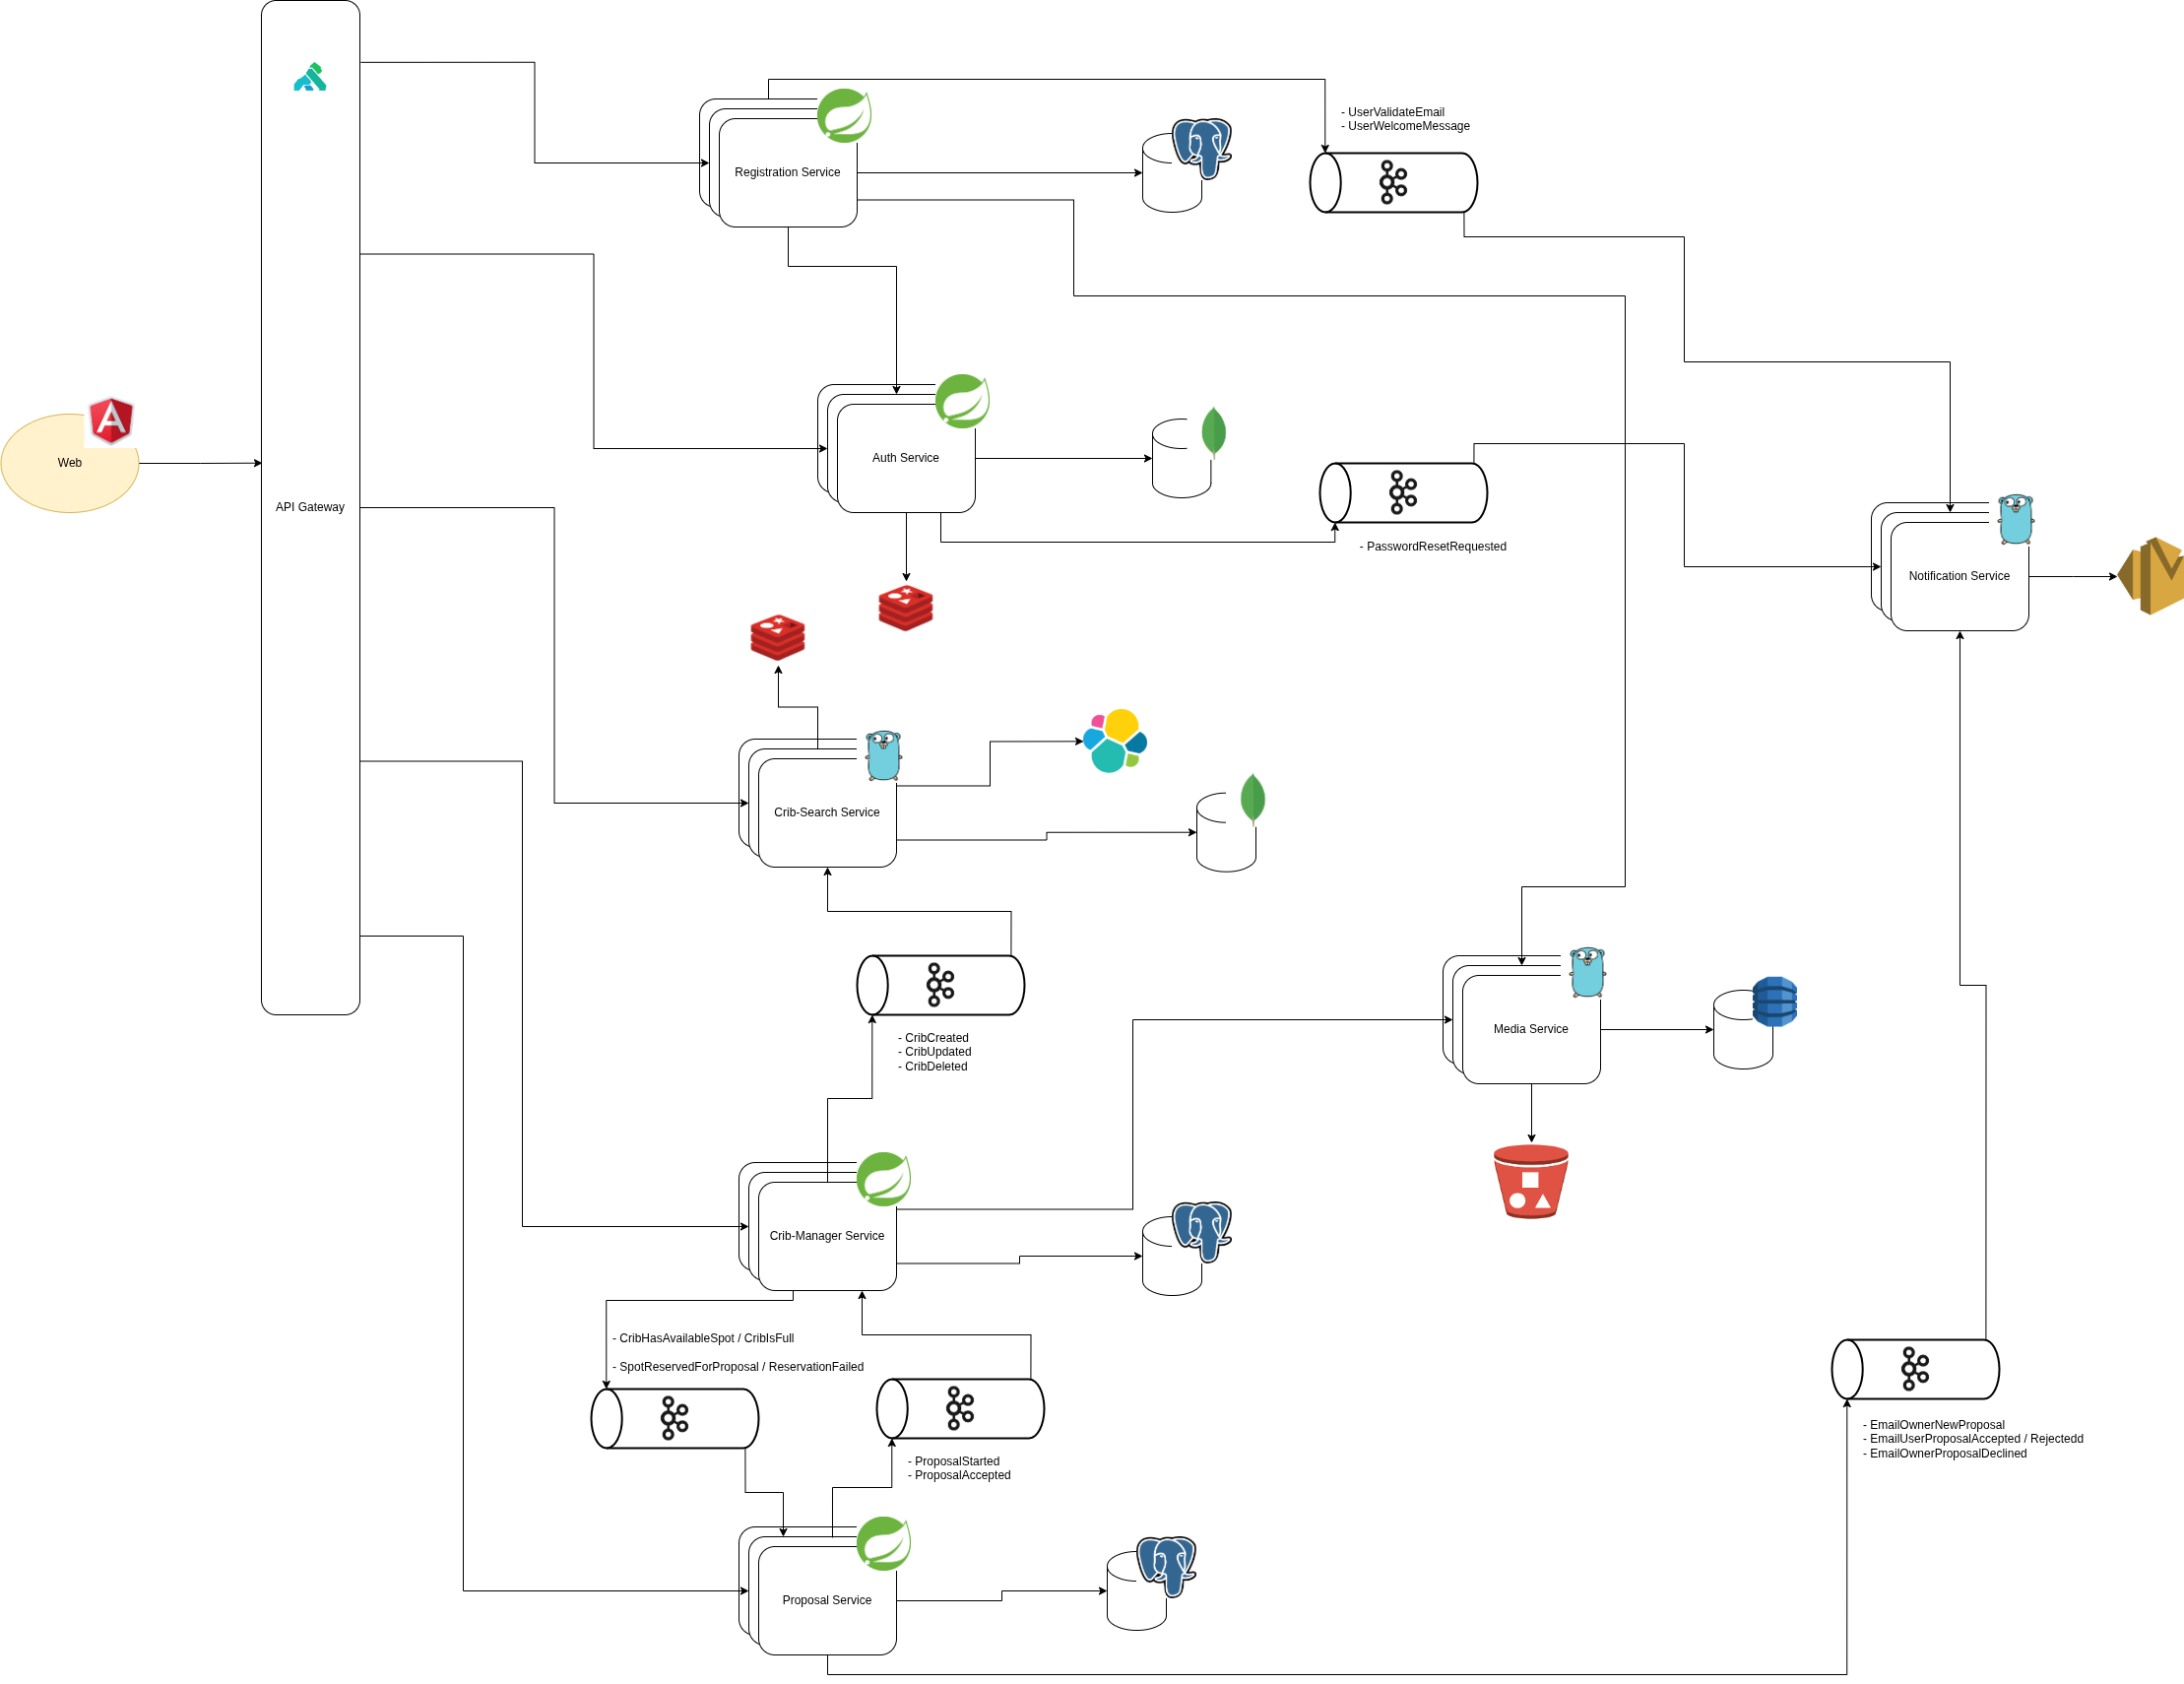
\includegraphics[width=0.8\textwidth]{figuras/campuscrib-diagram-system-design-macro.drawio.png}
	\caption{Arquitetura do Back-End do Sistema}
	\label{figura-arquitetura-campus}
\end{figure}



